\section{Internal} %{{{
\label{s:internal}

\subsection{Motivation}
Despite the emergence of various new types of storage devices developed in response to the increasing demand for high-performance and efficient storage solutions, the issue of fragmentation continues to persist in storage devices.
This problem of fragmentation can lead to degraded performance and aging of the storage devices.

When new research is conducted, new SSDs are expected to have the best performance with no fragmentation whatsoever. 
However, SSDs used in real life often experience performance degradation due to prolonged use and significant fragmentation. 
To address this, SSDs are aged to induce the desired level of fragmentation, allowing for a more accurate representation of the conditions in which SSDs are used.

In the case of HDDs, aging is relatively straightforward because the physical area and logical area coincide. 
In contrast, SSDs cannot be accessed externally due to security reasons related to the Flash Translation Layer (FTL), necessitating indirect aging.
This means that researchers cannot directly modify data placement and must perform aging by reading and writing meaningless data to the SSD for several days. 
This process is time-consuming and difficult to incorporate into research.

This motivation led to the idea of reducing the time required for aging by directly aging the SSD, retrieving data from the FTL, and storing it in files.
These files can then be loaded into the FTL of a new SSD to quickly configure an aged SSD. 
To achieve this, we attempted to store the FTL information and storage space data of a virtual SSD on a storage emulator called NVMeVirt, allowing for loading into a new SSD.
We argue that this approach will significantly reduce the time spent on aging tasks conducted to align with the actual user environment before research, making it an essential tool for researchers.
\begin{figure}[!t]
    \centering
    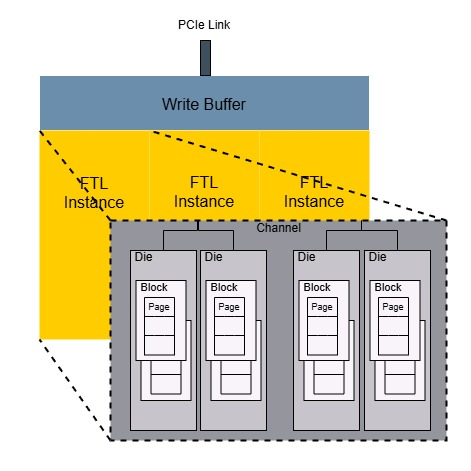
\includegraphics[width=0.5\textwidth,keepaspectratio]{figs/SSD structure.jpg}
    \caption{NVMeVirt SSD Structure}
    \label{fig:structure}
\end{figure}
\begin{figure}[!t]
    \centering
    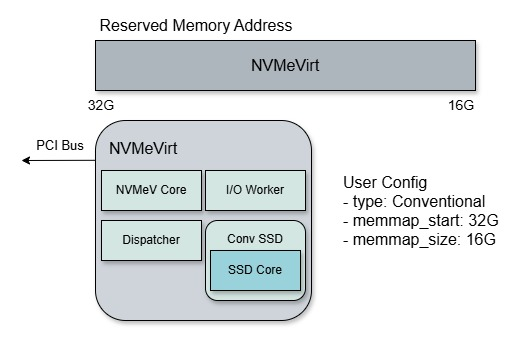
\includegraphics[width=0.5\textwidth,keepaspectratio]{figs/NVMeVirt making.jpg}
    \caption{Make the NVMeVirt Instance}
    \label{fig:making}
\end{figure}

\subsection{NVMeVirt}
NVMeVirt\cite{nvmevirt} is a Linux kernel module that provides a virtual NVMe device to the system, supporting various types of SSDs including basic SSDs, ZNS SSDs, and key-value SSDs. 
The device is emulated at the PCI layer and can be used not only for standard devices but also for advanced storage configurations such as NVMe-over-Fabrics offloads.

The storage space of modern SSDs is divided into multiple partitions, as shown in Figure \ref{fig:structure}, with each partition managed by a separate FTL instance. 
As a result, multiple FTL instances exist within a single SSD, sharing one PCIe link connected to the host.
Each partition consists of several NAND channels, and each channel is connected to multiple dies. 
This architecture allows for data transfer through NAND channels to be serialized, while each die can operate independently. 
In this structure, the FTL coordinates the dies and channels to handle I/O requests.
Thanks to this design, a single I/O request can be split into smaller tasks and distributed across multiple FTL instances, allowing for parallel processing.

As the data density per cell increases, the NAND programming time has also increased.
To hide this time, a write buffer is employed. The data from incoming write requests is stored in the write buffer, and the write request is considered complete when the payload is copied to the write buffer. 
If this write buffer becomes full, the data must be processed. 
However, in NVMeVirt, to facilitate one-shot programming, this data is not immediately processed. 
Instead, it waits until the buffering of another logical page in the same physical page is completed, after which the data is moved to the corresponding FTL for storage.
Once the write operation is complete, the FTL instance is reclaimed. 
This processing occurs in the background. 
For reads, the data is sent directly from the FTL instance to the buffer specified in the NVMe command without passing through the write buffer.

The storage of NVMeVirt is located in memory. 
Since a significant amount of memory is required for data storage, it is necessary to reserve a portion of the physical address space at system initialization through boot parameters, as shown in Figure \ref{fig:making}. 
Additionally, a simple linear mapping is used for data placement based on a conventional SSD. 
Therefore, the memory location for the physical block and page numbers in the flash address space is calculated by adding the starting address of the reserved memory area.

There are several tools available for simulating or emulating SSDs. 
Simulators use data processing models to mimic the internal operations of actual devices. 
Their primary purpose is to construct models of the devices and parameterize the performance of internal operations to calculate desired performance metrics in the model.
As a result, while detailed analysis is possible, executing actual workloads can slow down the overall system when simulating the entire system.

Many emulators similar to NVMeVirt exist; for instance, FlexDrive can only emulate existing SSD types and does not support devices like KVSSDs and ZNS SSDs. 
Our research aimed to reduce the time required for aging when conducting new studies, so we sought an emulator that could be used across various devices and thus did not utilize those emulators.
FEMU, on the other hand, provides a virtual NVMe device to guest operating systems by leveraging device virtualization features.
However, in a virtual machine environment, the guest physical memory is scattered across the host's physical memory through the host's virtual memory system, which can be inconvenient, and there is also the hassle of needing to reboot during experiments.

In contrast, NVMeVirt allows developers to easily modify the NVMe interface layer, enabling exploration of various design spaces and support for new device types.
Additionally, because it does not rely on virtualization technology, it permits comprehensive communication models with low overhead, and its modular design allows for easy usage through module loading.
For these reasons, we conducted our research on NVMeVirt.

Using an emulator like NVMeVirt enables direct access to the FTL, making our research feasible.
Through our research, we aim to facilitate the rapid creation of aged SSDs for future studies.

\begin{figure*}[!t]
    \centering
    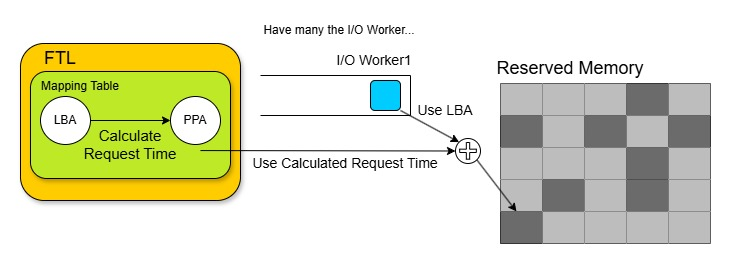
\includegraphics[width=0.9\textwidth,keepaspectratio]{figs/FTL's mapping table.jpg}
    \caption{NVMeVirt’s relation between FTL and data save process}
    \label{fig:mappingtable}
\end{figure*}
\begin{figure}[!t]
    \centering
    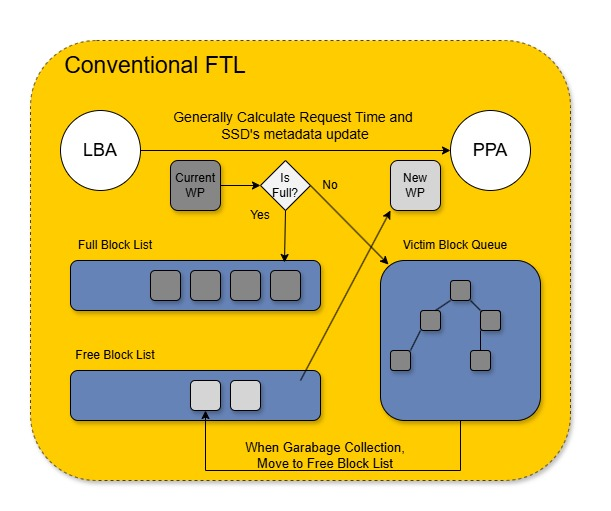
\includegraphics[width=0.5\textwidth,keepaspectratio]{figs/FTL role.jpg}
    \caption{FTL’s role}
    \label{fig:role}
\end{figure}

\subsection{Implementation}
\subsubsection{What to Bring}
There are four main types of data that need to be retrieved from the aged SSD on NVMeVirt. 
First, the metadata of the SSD related to the FTL must be obtained. 
Unlike actual SSDs, the FTL in NVMeVirt primarily performs the task of calculating request times. 
When storing data in actual storage, it uses Logical Block Addresses (LBA) instead of Physical Page Addresses (PPA), eliminating the need to convert LBA to PPA for disk I/O assistance. 
Instead, as shown in Figure \ref{fig:mappingtable}, the LBA is abstractly related to the PPA, and the expected request time is calculated so that the time taken to store or read data matches the computed request time.
This allows for abstract handling of each PPA.
Therefore, it is necessary to store the mapping table, reverse mapping table, and various parameters used to calculate request times.

Second, we need to bring the Free Block list, Full Block list, and Victim Block queue that manage the Free and Full blocks. 
The state of an SSD's blocks is divided into two categories: Full Blocks, which are completely written, and Free Blocks, which are empty. 
The FTL manages these blocks in list form. 
As shown in Figure \ref{fig:role}, when the LBA is converted to PPA within the FTL and the request time is calculated, the write pointer is placed in either the Victim Block queue or the Full Block List.
The Victim Block queue contains blocks that have data written but are not yet in the Full Block state. 
Later, through Garbage Collection, the data in these blocks is cleared to transition them to Free Block status. 
The FTL manages Free Blocks through the Free Block List, allocating blocks from this list whenever a new write pointer is needed.
In other words, the state of the SSD blocks is managed through the Free Block List, Full Block List, and Victim Block queue, which determines where to write data. 
Therefore, it is essential to preserve this data regarding block states.

Third, metadata about the SSD itself, beyond the FTL, must be retrieved. 
Since NVMeVirt is an emulator for SSDs, it manages metadata for channels, blocks, and pages.
Most of this data can be recreated in a new SSD without issues. 
However, metadata for blocks and especially pages must be retained.
The page metadata includes the status of each page, which distinguishes whether the page is in a valid or invalid state. 
When a new SSD is created, all pages are initialized to a valid state, so this information must be preserved. 
For blocks, the metadata includes the count of valid pages, the count of invalid pages, and the erase count.
This information also needs to be maintained, as it will be reset in the new SSD.
Failing to retain the metadata for pages and blocks could lead to conflicts with the FTL's metadata, resulting in issues.

Lastly, the contents of the storage must be retrieved.
The storage in NVMeVirt exists linearly in memory. To obtain the contents of the storage, it is necessary to copy from the starting address of the storage for the entire size of the storage.

\subsubsection{ How to Save and Load}
To maintain the data mentioned in Section 3.3.1 in the new SSD, it must be saved to external files and then loaded into the new SSD. 
However, since NVMeVirt is a kernel module, this requires reading from and writing to files in User Space from the kernel space.
Generally, reading and writing files from kernel space to User Space is not recommended due to reasons such as kernel protection and over-reliance on User Space.
Nonetheless, in this research, the advantages gained from reading and writing files from kernel space outweigh the drawbacks, so we proceeded with this approach.


As mentioned in Section 3.3.1, the data that needs to be preserved includes the FTL metadata, block lists, SSD storage metadata, and contents. 
Instead of managing these in multiple files, we opted to store them in a single file for convenience in later distribution and SSD aging creation.
The functions used for reading and writing to the file are Kernel\_Write() and Kernel\_Read().


There are two key points to highlight. 
First is the block lists.
The FTL manages blocks in list form. Since the mapping table is created as an array, the entire array can simply be copied.
However, for linked lists, this is not possible.
To copy a linked list, we must traverse the list and save the information in order.
Care must also be taken during loading; in the new SSD, all blocks exist in a Free Block state and are included in the Free Block List. 
Even if multiple read and write operations have been conducted on the new SSD, the blocks included in the Free Block List and Full Block List will differ from those in the aged SSD. 
Therefore, all lists must be initialized before loading.


The second point is the storage data saving process. 
While the storage may contain contents across all ranges, it may also have empty spaces.
If we were to save the entire range of the storage to the file, it could include empty spaces, making it inefficient.
Thus, we aim to skip the empty spaces and only save the areas where data is present in the file. 
This can be easily implemented using the mapping table. 
The mapping table is stored in an array format, with the index representing the Logical Page Number (LPN) and the stored value representing the Physical Page Number (PPA).
NVMeVirt uses the LPN to store data in the storage and can verify whether data is stored in a given page using the PPA. 
Therefore, by traversing the mapping table, we check whether data is stored in the page via the PPA, and if it is, we save the page's size to the file using the LPN.


The loading process also utilizes the mapping table.
Similarly, since the data for the mapping table is saved and loaded together with the file, we can confirm the pages using the PPA and attempt to load the data into storage using the LPN. 
This approach allows us to avoid storing unnecessary data, thereby reducing the file size for distribution and saving time.
